\chapter{Einführung}
Das Michelson Interferometer bezeichnet einen Versuchsaufbau, der auch heute noch Verwendung findet. Sein Mechanismus besteht darin kohärentes Licht aufzuspalten und nach Durchlauf zweier verschiedener Pfade wieder zu vereinen. Zwischen den beiden Pfaden wird durch Änderung des optischen Weges ein Phasenunterschied zwischen den betreffenden Lichtstrahlen erzeugt. Da sich elektrische Felder in einer Superposition addieren, lässt die Phasendifferenz ein Interferenzmuster entstehen, das genutzt werden kann, um Aussagen über das verwendete Licht oder die optischen Wege zu treffen.
\begin{figure}[H]
    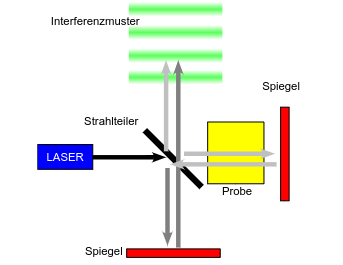
\includegraphics{pictures/ms_interferometer_aufbau.png}\label{fig:aufbau}
    \caption{\textbf{Aufbau eines Michelson Interferometers.} Das Bild ist der Versuchsanleitung entnommen.}
\end{figure}
In \figref{fig:aufbau} wird ein schematischer Aufbau eines Michelson Interferometers gezeigt. Ein Laser stellt einen kohärenten Lichtstrahl zur Verfügung. Dieser wird an einem Strahlteiler zu gleichen Teilen auf zwei unterschiedliche Wege geschickt. Der optische Wegunterschied zwischen den Pfaden kann über den Abstand der beiden Spiegel gesteuert werden, welche das Licht wieder zurück schicken. Außerdem kann ein Medium in einen der Strahlen eingeführt werden, der den optischen Weg zusätzlich verändert. Nach der Spiegelung der Strahlen laufen diese im Strahlteiler wieder zusammen und werden vereint auf ein Auswertungselement geschickt. In unserem Fall ist dies ein Schirm oder eine Photodiode. Flächen mit gleicher optischen Wegdifferenz besitzen die gleiche Fläche. Im Fall von parallelem Licht, bzw. ebenen Wellen, sind dies Ebenen, während es für Kugelwellen entsprechend Kugelflächen sind. Folglich bildet das Interferenzmuster auf dem Schirm für paralleles Licht Linien und für Kugelwellen Kreise. Das Einführen von Sammel- und Streulinsen in den Laserstrahl kann paralleles Licht in Kugelwellen umwandeln.
\begin{figure}[H]\label{fig:beugung_ebene}
    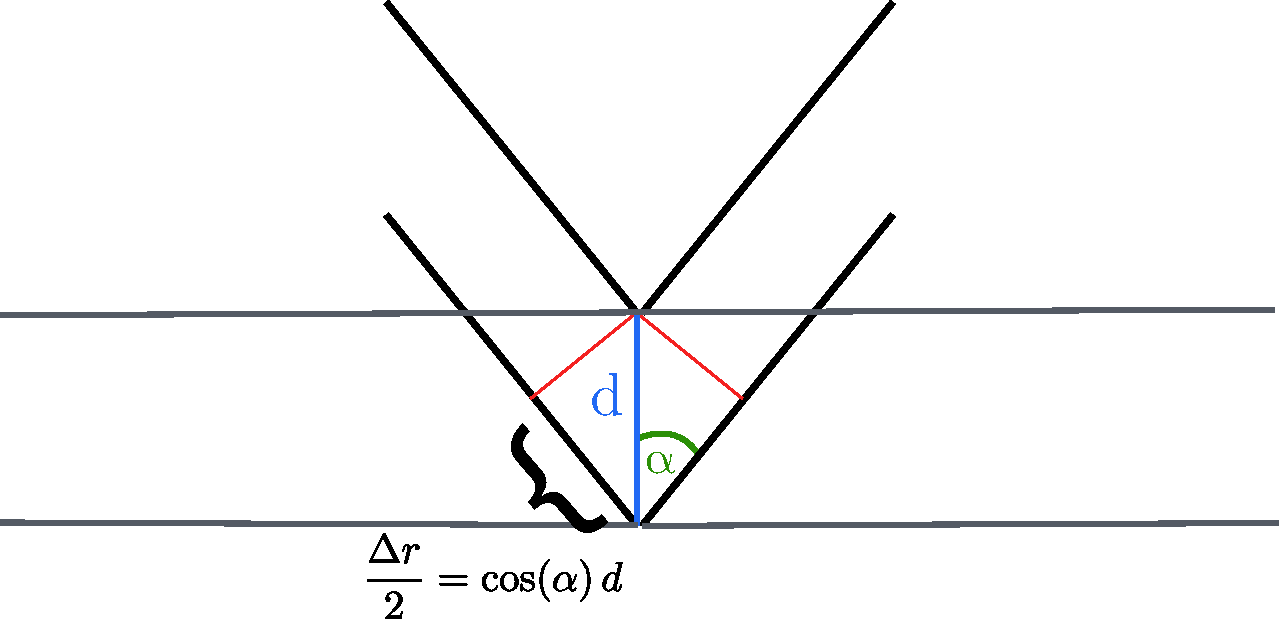
\includegraphics[scale=0.7]{pictures/path3.pdf}\label{fig:aufbau}
    \caption{\textbf{Wegunterschied zwischen den beiden Strahlen.} Die oberen beiden horizontalen Linien stellen die Spiegel dar. Diese sind so gegeneinander verschoben, dass sich der Länge des Weges zwischen beiden Pfaden für horizontale Strahlen um die Distanz $2\cdot d$ unterscheidet. Der Winkel $\alpha$ gibt die Abweichung des Wellenvektors von einer horizontalen Richtung an.}
\end{figure}
Für den Fall das sich der optische Weg der beiden Pfade nur um eine Differenz in der Spiegelposition $d$ unterscheidet, berechnet sich die Phasendifferenz in Abhängigkeit des Winkels zwischen Mittelpunkt des Schirms und eines Punktes freier Wahl, gemäß \figref{fig:beugung_ebene}, zu
\begin{align*}\label{eq:phasendiff_ebenen}
    2\pi n\overset{!}{=}\Delta\varphi&=k\,\cos(\alpha)\,d\quad n\in\mathbb{N}\\
    \Rightarrow\quad n\cdot\lambda&=\cos(\alpha)\,d
\end{align*}